【楽曲再生】
\par
%ここから本文
選曲アルゴリズムによりリスト化された楽曲を再生する.機能では,再生ボタン,一時停止ボタン,次の楽曲に遷移するボタン,
前の楽曲に遷移するボタンがあり,タップをすれば各機能が動作する.機能については次の項目で詳しく説明する.
\par
【UI】
\par
%ここから本文
画面は音楽再生画面と優先度設定を行う画面の2つがある(図 3.1).優先度設定に関しては次の項目で詳しく説明する.両画面とも右下の矢印のボタンをタップするとそれぞれ画面遷移が起こる.まず,優先度設定画面では5つの要素があり,BPMをON/OFFで分けるトグルスイッチを利用し,他の4つの要素(天気,時間,場所,季節)にはシークバーを利用した.デフォルト設定ではつまみの位置は中心の置かれ,右側に移動させるほど優先され,選曲に考慮される.各要素では分かりやすいように各シークバーに配色した.シークバーの上にあるテキストはユーザのシチュエーションから情報を取得し,各要素に現在のシチュエーションを表示している.音楽再生画面では上記にあるようにボタンが配置されている.中央にあるテキストは流れている楽曲のタイトル,歌手,曲の長さが表示される.またそれを囲むようにある円は,一曲で円の軌跡にあるちいさなつまみが一周する様になっており音楽再生位置を表している.また手動で再生位置をかえる事ができる仕様にするつもりではあったが,開発に手こずり未だ実装できていない.
\par
画面は情報量を極力なくし,シンプルなデザインを心がけた.優先度設定画面では各要素した配色を際立たせるために背景を白くし,音楽再生画面では優先度設定画面とは違い落ち着いた色の黒を背景にし,音楽の象徴である音符を中央に配置した.音楽再生画面では目をくらませないよう,青を基調とした配色をした.

\begin{center}
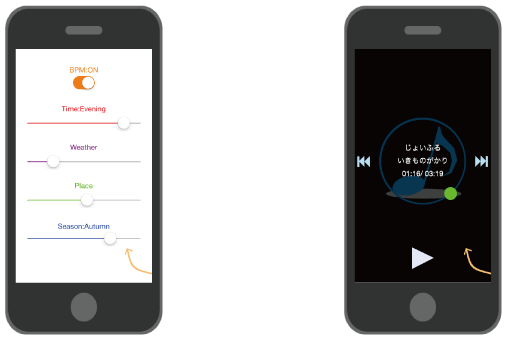
\includegraphics[width=5cm, bb=0 0 200 150]{UI.png}\\図 3.1: 優先度設定画面(左)と音楽再生画面(右)のUI
\end{center}

\bunseki{中司 智朱希(未来大)}
